\documentclass[aspectratio=1610, xcolor=table]{beamer}

%%% LATEX COLORS (OPENCOLORS)
%%% 2020
%%%%%%%%%%%%%%%%%%%%%%%%%%%%%%%

% GRAY
\definecolor{gray0}{HTML}{f8f9fa}
\definecolor{gray1}{HTML}{f1f3f5}
\definecolor{gray2}{HTML}{e9ecef}
\definecolor{gray3}{HTML}{dee2e6}
\definecolor{gray4}{HTML}{ced4da}
\definecolor{gray5}{HTML}{adb5bd}
\definecolor{gray6}{HTML}{868e96}
\definecolor{gray7}{HTML}{495057}
\definecolor{gray8}{HTML}{343a40}
\definecolor{gray9}{HTML}{212529}

% RED
\definecolor{red0}{HTML}{fff5f5}
\definecolor{red1}{HTML}{ffe3e3}
\definecolor{red2}{HTML}{ffc9c9}
\definecolor{red3}{HTML}{ffa8a8}
\definecolor{red4}{HTML}{ff8787}
\definecolor{red5}{HTML}{ff6b6b}
\definecolor{red6}{HTML}{fa5252}
\definecolor{red7}{HTML}{f03e3e}
\definecolor{red8}{HTML}{e03131}
\definecolor{red9}{HTML}{c92a2a}

% PINK
\definecolor{pink0}{HTML}{fff0f6}
\definecolor{pink1}{HTML}{ffdeeb}
\definecolor{pink2}{HTML}{fcc2d7}
\definecolor{pink3}{HTML}{faa2c1}
\definecolor{pink4}{HTML}{f783ac}
\definecolor{pink5}{HTML}{f06595}
\definecolor{pink6}{HTML}{e64980}
\definecolor{pink7}{HTML}{d6336c}
\definecolor{pink8}{HTML}{c2255c}
\definecolor{pink9}{HTML}{a61e4d}

% GRAPE
\definecolor{grape0}{HTML}{f8f0fc}
\definecolor{grape1}{HTML}{f3d9fa}
\definecolor{grape2}{HTML}{eebefa}
\definecolor{grape3}{HTML}{e599f7}
\definecolor{grape4}{HTML}{da77f2}
\definecolor{grape5}{HTML}{cc5de8}
\definecolor{grape6}{HTML}{be4bdb}
\definecolor{grape7}{HTML}{ae3ec9}
\definecolor{grape8}{HTML}{9c36b5}
\definecolor{grape9}{HTML}{862e9c}

% VIOLET
\definecolor{violet0}{HTML}{f3f0ff}
\definecolor{violet1}{HTML}{e5dbff}
\definecolor{violet2}{HTML}{d0bfff}
\definecolor{violet3}{HTML}{b197fc}
\definecolor{violet4}{HTML}{9775fa}
\definecolor{violet5}{HTML}{845ef7}
\definecolor{violet6}{HTML}{7950f2}
\definecolor{violet7}{HTML}{7048e8}
\definecolor{violet8}{HTML}{6741d9}
\definecolor{violet9}{HTML}{5f3dc4}

% INDIGO
\definecolor{indigo0}{HTML}{edf2ff}
\definecolor{indigo1}{HTML}{dbe4ff}
\definecolor{indigo2}{HTML}{bac8ff}
\definecolor{indigo3}{HTML}{91a7ff}
\definecolor{indigo4}{HTML}{748ffc}
\definecolor{indigo5}{HTML}{5c7cfa}
\definecolor{indigo6}{HTML}{4c6ef5}
\definecolor{indigo7}{HTML}{4263eb}
\definecolor{indigo8}{HTML}{3b5bdb}
\definecolor{indigo9}{HTML}{364fc7}

% BLUE
\definecolor{blue0}{HTML}{e7f5ff}
\definecolor{blue1}{HTML}{d0ebff}
\definecolor{blue2}{HTML}{a5d8ff}
\definecolor{blue3}{HTML}{74c0fc}
\definecolor{blue4}{HTML}{4dabf7}
\definecolor{blue5}{HTML}{339af0}
\definecolor{blue6}{HTML}{228be6}
\definecolor{blue7}{HTML}{1c7ed6}
\definecolor{blue8}{HTML}{1971c2}
\definecolor{blue9}{HTML}{1864ab}

% CYAN
\definecolor{cyan0}{HTML}{e3fafc}
\definecolor{cyan1}{HTML}{c5f6fa}
\definecolor{cyan2}{HTML}{99e9f2}
\definecolor{cyan3}{HTML}{66d9e8}
\definecolor{cyan4}{HTML}{3bc9db}
\definecolor{cyan5}{HTML}{22b8cf}
\definecolor{cyan6}{HTML}{15aabf}
\definecolor{cyan7}{HTML}{1098ad}
\definecolor{cyan8}{HTML}{0c8599}
\definecolor{cyan9}{HTML}{0b7285}

% TEAL 
\definecolor{teal0}{HTML}{e6fcf5}
\definecolor{teal1}{HTML}{c3fae8}
\definecolor{teal2}{HTML}{96f2d7}
\definecolor{teal3}{HTML}{63e6be}
\definecolor{teal4}{HTML}{38d9a9}
\definecolor{teal5}{HTML}{20c997}
\definecolor{teal6}{HTML}{12b886}
\definecolor{teal7}{HTML}{0ca678}
\definecolor{teal8}{HTML}{099268}
\definecolor{teal9}{HTML}{087f5b}

% GREEN
\definecolor{green0}{HTML}{ebfbee}
\definecolor{green1}{HTML}{d3f9d8}
\definecolor{green2}{HTML}{b2f2bb}
\definecolor{green3}{HTML}{8ce99a}
\definecolor{green4}{HTML}{69db7c}
\definecolor{green5}{HTML}{51cf66}
\definecolor{green6}{HTML}{40c057}
\definecolor{green7}{HTML}{37b24d}
\definecolor{green8}{HTML}{2f9e44}
\definecolor{green9}{HTML}{2b8a3e}

% LIME
\definecolor{lime0}{HTML}{f4fce3}
\definecolor{lime1}{HTML}{e9fac8}
\definecolor{lime2}{HTML}{d8f5a2}
\definecolor{lime3}{HTML}{c0eb75}
\definecolor{lime4}{HTML}{a9e34b}
\definecolor{lime5}{HTML}{94d82d}
\definecolor{lime6}{HTML}{82c91e}
\definecolor{lime7}{HTML}{74b816}
\definecolor{lime8}{HTML}{66a80f}
\definecolor{lime9}{HTML}{5c940d}

% YELLOW
\definecolor{yellow0}{HTML}{fff9db}
\definecolor{yellow1}{HTML}{fff3bf}
\definecolor{yellow2}{HTML}{ffec99}
\definecolor{yellow3}{HTML}{ffe066}
\definecolor{yellow4}{HTML}{ffd43b}
\definecolor{yellow5}{HTML}{fcc419}
\definecolor{yellow6}{HTML}{fab005}
\definecolor{yellow7}{HTML}{f59f00}
\definecolor{yellow8}{HTML}{f08c00}
\definecolor{yellow9}{HTML}{e67700}

% ORANGE
\definecolor{orange0}{HTML}{fff4e6}
\definecolor{orange1}{HTML}{ffe8cc}
\definecolor{orange2}{HTML}{ffd8a8}
\definecolor{orange3}{HTML}{ffc078}
\definecolor{orange4}{HTML}{ffa94d}
\definecolor{orange5}{HTML}{ff922b}
\definecolor{orange6}{HTML}{fd7e14}
\definecolor{orange7}{HTML}{f76707}
\definecolor{orange8}{HTML}{e8590c}
\definecolor{orange9}{HTML}{d9480f}

\usepackage{graphicx}
\usepackage{xcolor}
\graphicspath{{graphics/}}
\usepackage{listings,bera}
\usepackage[binary-units]{siunitx}
\usepackage{fontspec}
\usepackage{tgheros}
\usepackage{inconsolata}
\usetheme{bjeldbak}

\setmainfont{TeX Gyre Heros}

\setmonofont{Inconsolatazi4}
\lstset{
  language=Matlab,
  basicstyle=\ttfamily,
  keywordstyle=\bfseries\color{cyan5},
  identifierstyle=\color{black},
  rulecolor=\color{gray1},
  frame=single,
  frameround=tttt,
  %framesep=1.382em,
  backgroundcolor=\color{gray0},
}

\newcommand{\smallemskip}{
  \vspace{0.145898em}
}
\newcommand{\medemskip}{
  \vspace{0.382em}
}
\newcommand{\bigemskip}{
  \vspace{0.618em}
}
\newcommand{\smallgrskip}{
  \vspace{0.0901699\paperheight}
}
\newcommand{\medgrskip}{
  \vspace{0.145898\paperheight}
}
\newcommand{\biggrskip}{
  \vspace{0.236067978\paperheight}
}

% 1: first column content
% 2: second column content
% 3: width of first column
\newcommand{\twocolumns}[3]{
    \begin{columns}
      \begin{column}{#3}
          #1
        \end{column}
        \begin{column}{\dimexpr(\textwidth-#3)}
          #2
        \end{column}
    \end{columns}
}


\title{Informationsübertragung}
\subtitle{Testataufgaben}
\author{Richard \color{hsblue}{\textsc{Grünert}}}
\institute{Hochschule Wismar}
\titlegraphic{
}

\begin{document}

{
  \setbeamertemplate{headline}{}
  \begin{frame}
    \twocolumns{
      \begin{center}
      
\includegraphics[width=0.618\textwidth]{logo}
    \end{center}
    }{

      \titlepage

    }{0.382\textwidth}
  \end{frame}
}

  % {%
  %   \setbeamertemplate{headline}{}
  %   \frame{\titlepage}
  % }
  \addtocounter{framenumber}{-1}

  \section{Aufgabe 1}
  \input{slides/Aufgabe1}

  \section{Aufgabe 2}
  \begin{frame}{Aufgabe 2: Basisband I}
  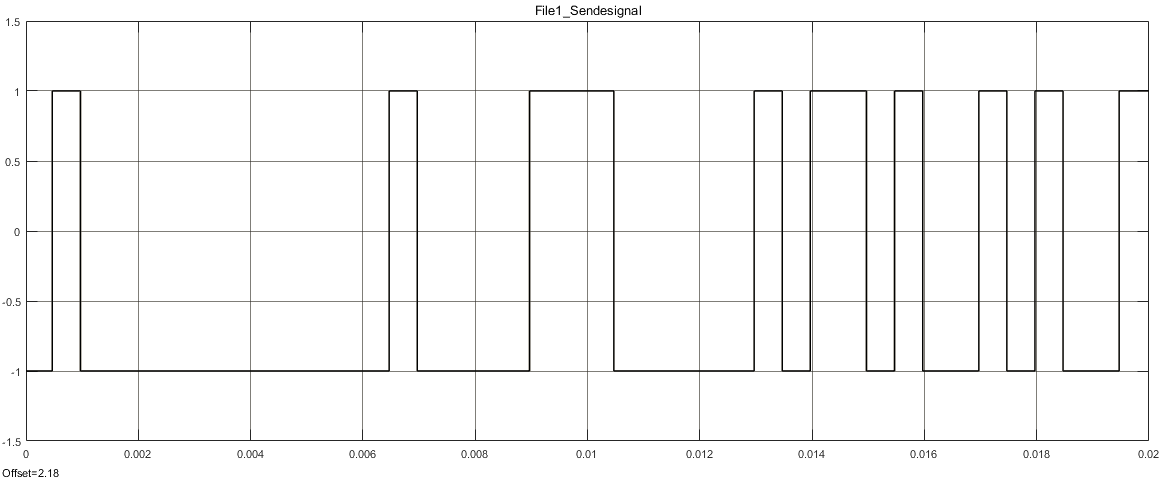
\includegraphics[width=\textwidth]{screenshots/Aufgabe2/Zeitsignal_File1}
\end{frame}

\begin{frame}{Aufgabe 2: Basisband I}
  \begin{center}
  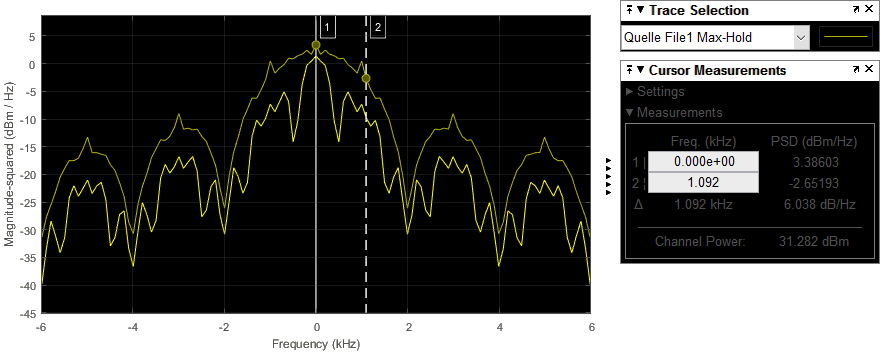
\includegraphics[height=0.4\textheight]{screenshots/Aufgabe2/Spektrum_File1}\\
  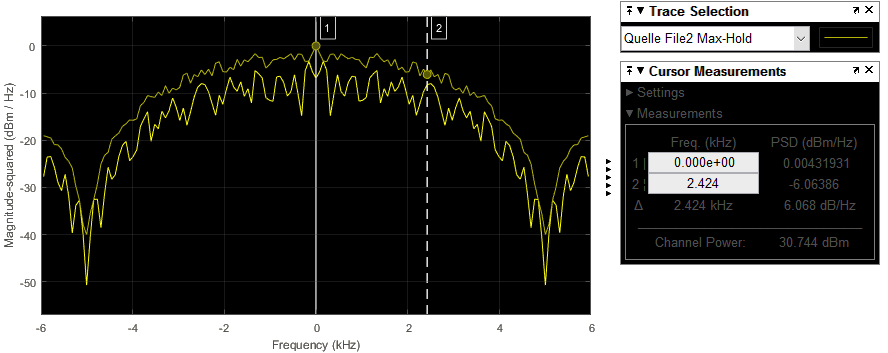
\includegraphics[height=0.4\textheight]{screenshots/Aufgabe2/Spektrum_File2}
  \end{center}
\end{frame}

\begin{frame}{Aufgabe 2: Basisband I}
  \begin{table}[H]
    \begin{tabular}{
      >{\columncolor{gray0}}l ll}
      Signal & \cellcolor{gray0}Datenrate (BR) & \cellcolor{gray0}Bandbreite ($6 \, \si{\deci\bel}$ (B)) \\
      \hline
      File 1 &  $2.001 \, \si{\kilo\bit\per\second}$                            & $1.092 \, \si{\kilo\hertz}$                              \\
      File 2    &  $5.006 \, \si{\kilo\bit\per\second}$                              &            $2.424 \, \si{\kilo\hertz}$                 
    \end{tabular}
  \end{table}

  \bigemskip
  
  Inetwa linearer Zusammenhang:\\
  \[B \approx \frac{1}{2} \cdot BR= \frac{1}{2} \cdot \frac{1}{T_S}\]
  
  \to \, Bandbreite bei $1 \, \si{\kilo\bit\per\second}$:
  \[B \approx \frac{1}{2} \cdot 1000 \, \si{\kilo\bit\per\second} = 500 \, \si{\hertz}\]
  
\end{frame}


  \section{Aufgabe 3}
  \begin{frame}{Aufgabe 3: Basisband II}
  \begin{center}
  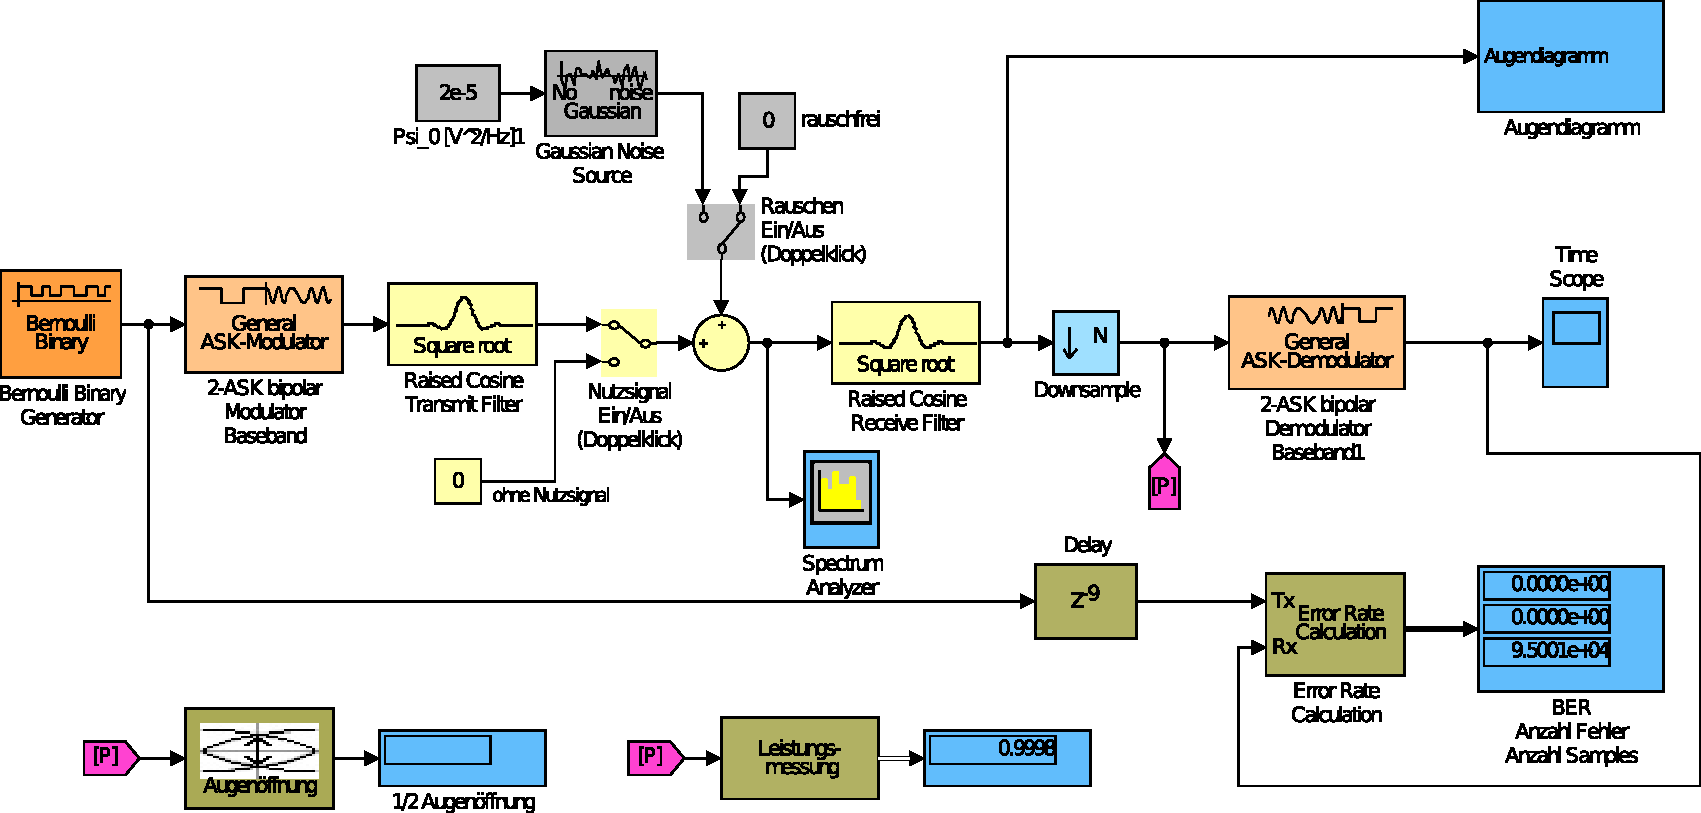
\includegraphics[width=\textwidth]{screenshots/Aufgabe3/modell}
  \end{center}
\end{frame}

\begin{frame}{Aufgabe 3: Basisband II}
  \twocolumns{
    \[B \approx 2.76 \, \si{\kilo\hertz}\]
    }{
      \begin{center}
  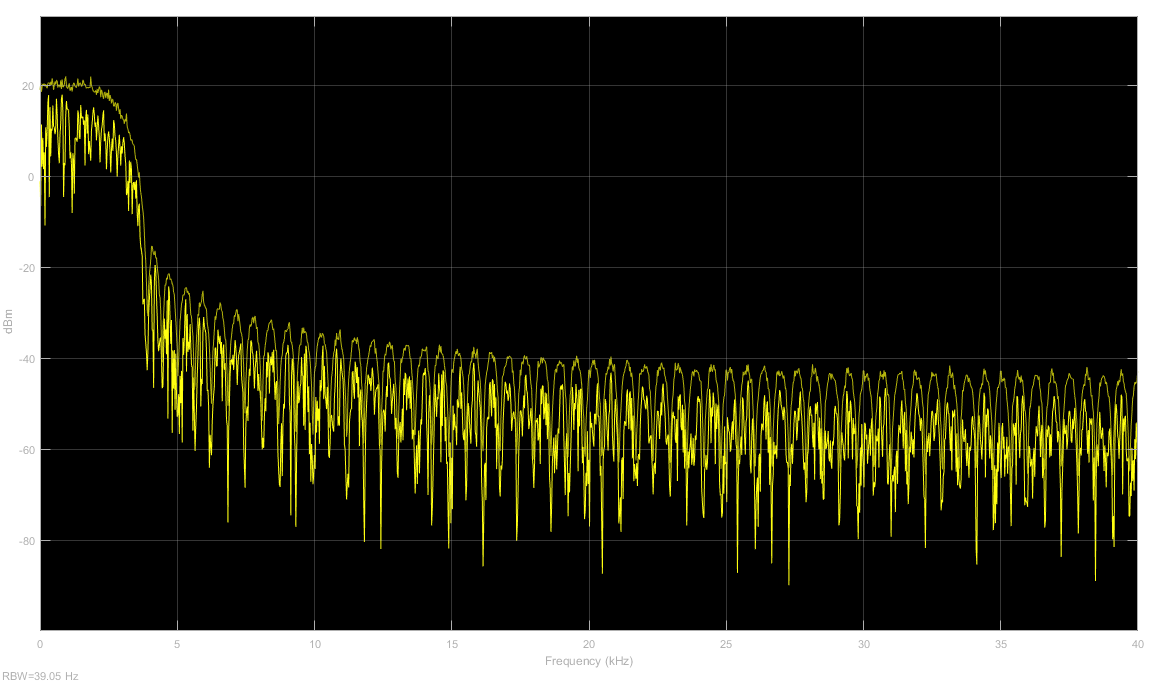
\includegraphics[width=0.854102\textwidth]{screenshots/Aufgabe3/spektrum_sendesignal}
  \end{center}
  }{0.0901699\textwidth}
\end{frame}

\begin{frame}{Aufgabe 3: Basisband II}
  \twocolumns{
    \[U_\mathrm{A} \approx 0.9965 \, \si{\volt}\]
    \[P_\mathrm{R} \approx 0.1 \, \si{\volt}^2\]
    }{
      \begin{center}
  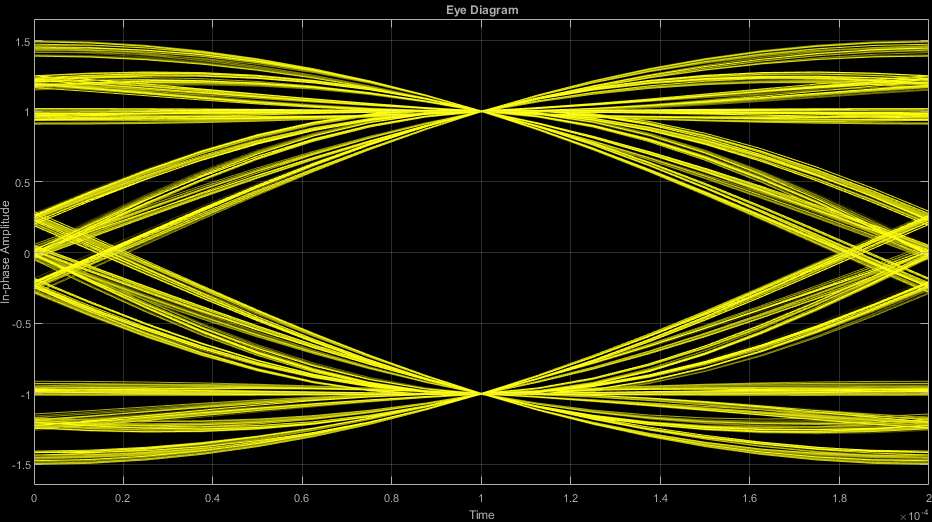
\includegraphics[width=0.854102\textwidth]{screenshots/Aufgabe3/auge_sendesignal}
  \end{center}
  }{0.0901699\textwidth}
\end{frame}

\begin{frame}{Aufgabe 3: Basisband II}
  \[\mathrm{BER} = \frac{1}{\log_2{s}} \cdot \frac{s-1}{s} \cdot
    \mathrm{erfc}{\left(\sqrt{\frac{\rho}{2}}\right)}, \, s = 2\]
  \[\mathrm{BER} = 0.5 \cdot \mathrm{erfc}{\left( \sqrt{\frac{9.93}{2}}
      \right)} = 8.1303 \cdot 10^{-4}\]
  gemessen:
  \[\mathrm{BER}_g = 8.86315 \cdot 10^{-4}\]
\end{frame}

  \section{Aufgabe 4}
  \begin{frame}{Aufgabe 4: Änderung des Empfangsfilters}
  % \twocolumns{
    \[B = 2.76 \, \si{\kilo\hertz}\]
    \[U_\mathrm{A}=0.8651 \, \si{\volt}\]
    \[P_\mathrm{R}=0.09861 \, \si{\volt}^2\]
    \[\rho = \frac{U_\mathrm{A}^2}{P_\mathrm{R}} = 7.59\]
    \[\textrm{BER} = 2.9 \cdot 10^{-3}\]
    \[\textrm{BER}_g = 1.7036 \cdot 10^{-3}\]
    % }{
  % \begin{center}
  % 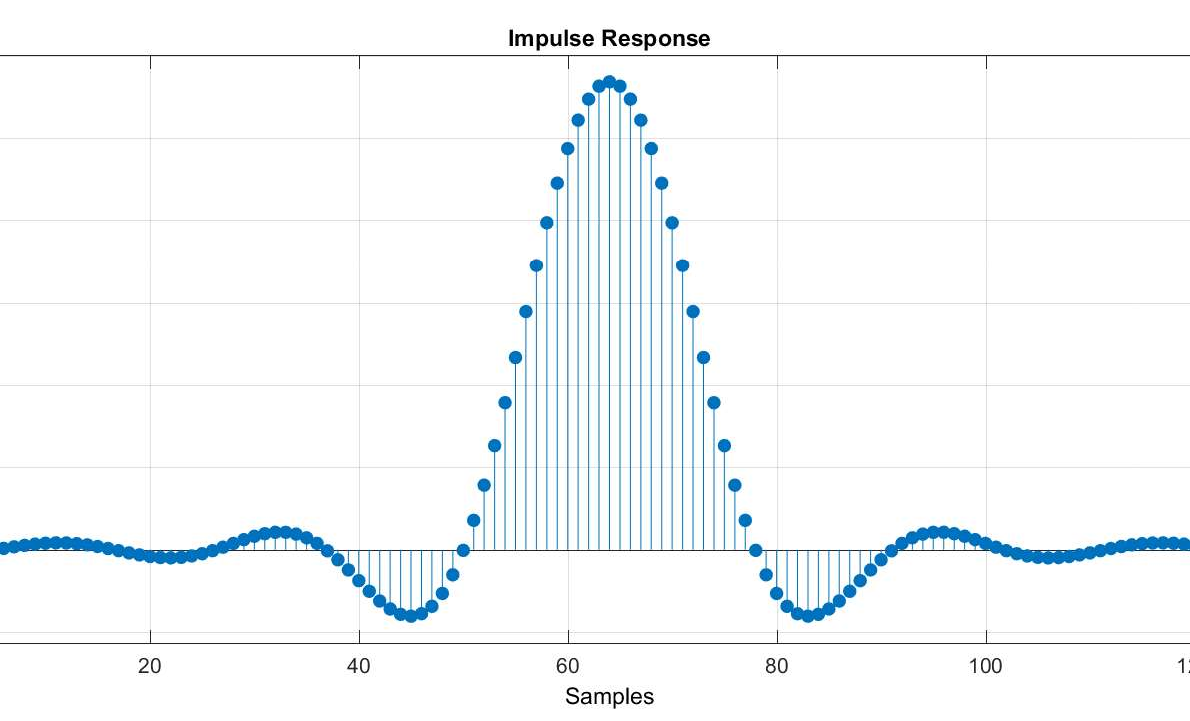
\includegraphics[width=\textwidth]{screenshots/Aufgabe4/sendefilter_impulsantwort}
  % \end{center}
  % }{0.5\textwidth}
\end{frame}

\begin{frame}{Aufgabe 4: Änderung des Empfangsfilters}
  \[g_{\mathrm{ef}}(t) \neq g_\mathrm{s}(-t)\]
\end{frame}

  \section{Aufgabe 5}
  \begin{frame}{Aufgabe 5: Nichtfrequenzselektive Bedingungen}

\twocolumns{
  
  \begin{center}
    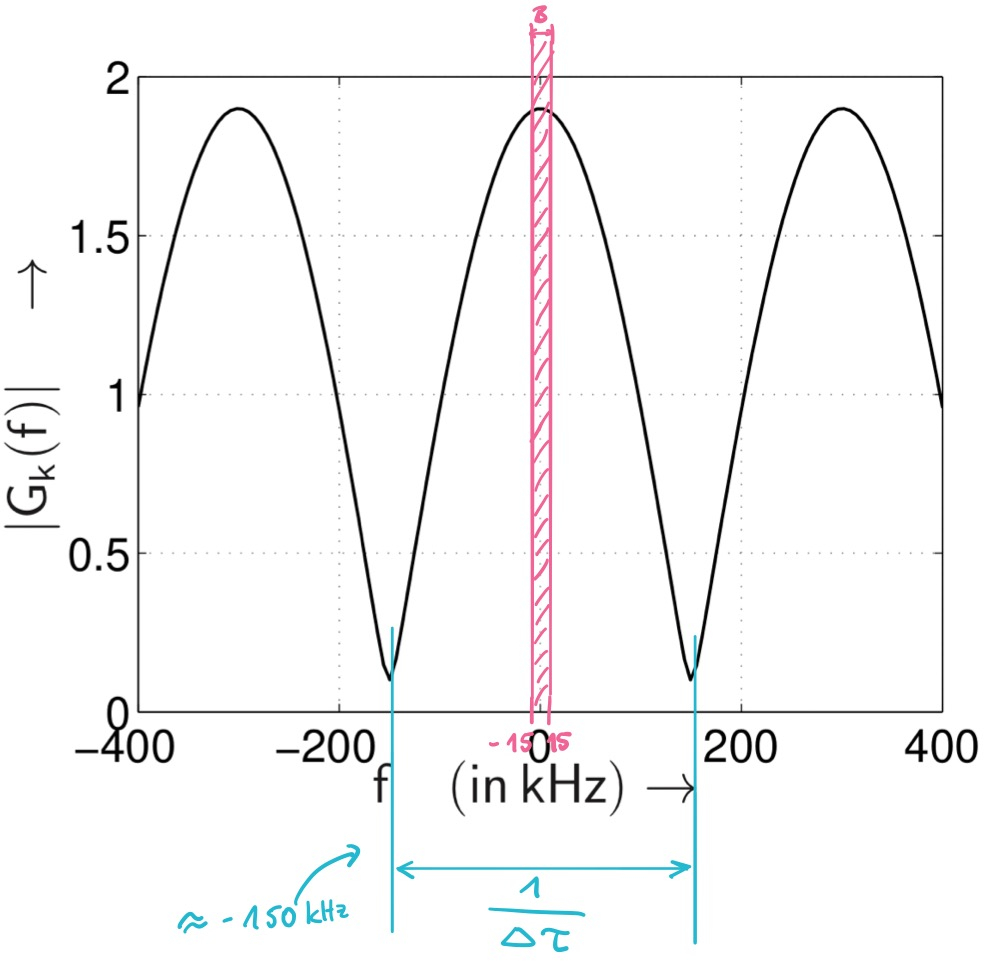
\includegraphics[width=\textwidth]{screenshots/Aufgabe5/1}
  \end{center}

}{

  \begin{center}
    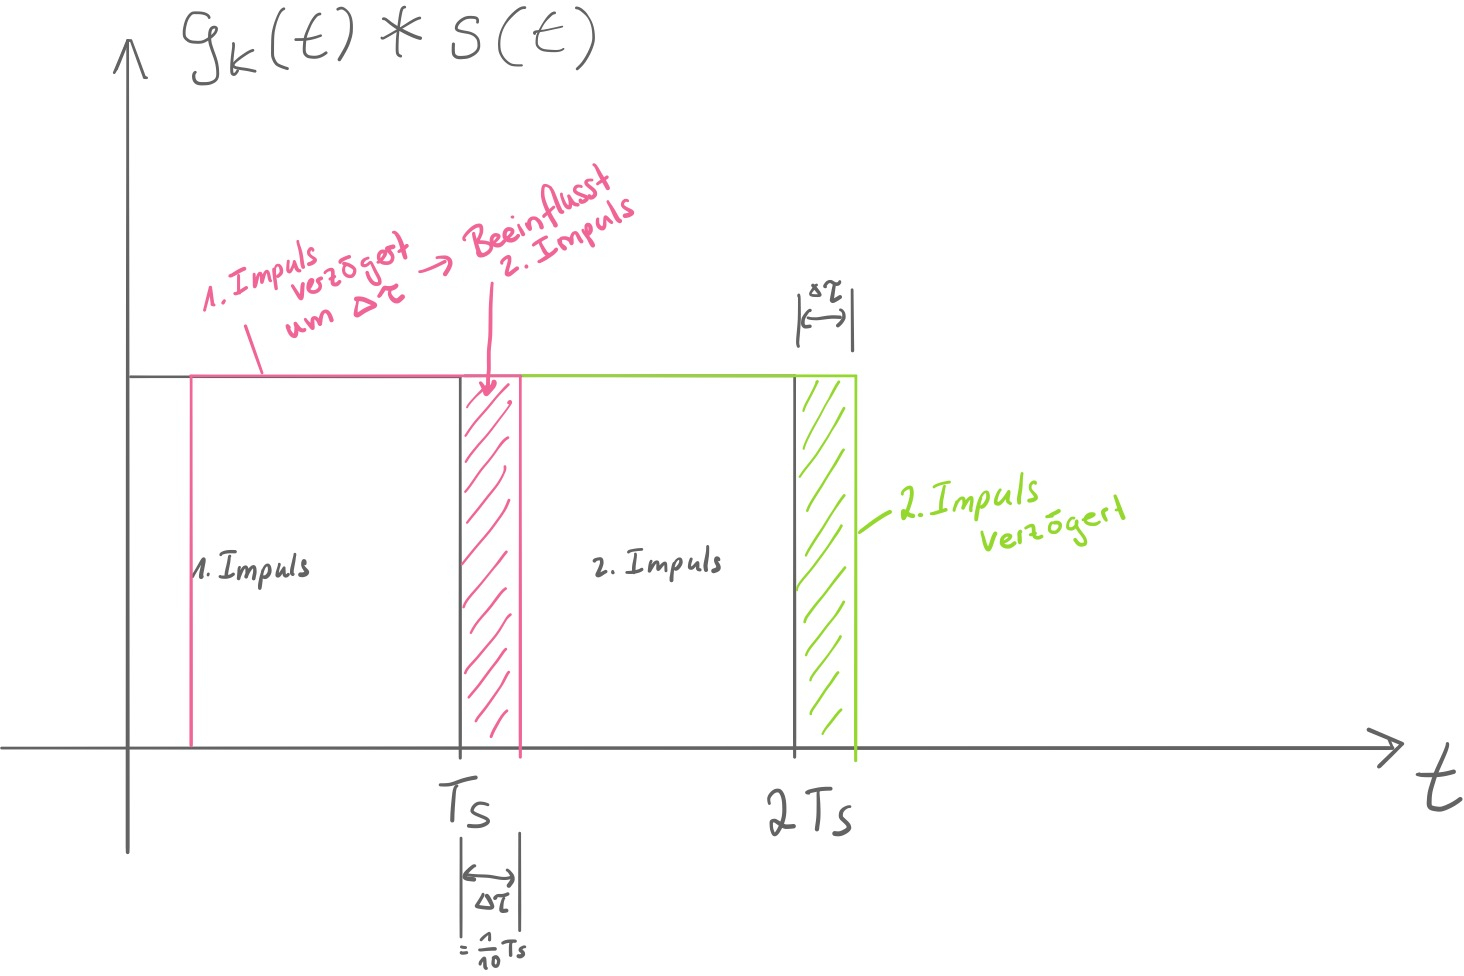
\includegraphics[width=\textwidth]{screenshots/Aufgabe5/2}
  \end{center}

  
}{0.5\textwidth}
\end{frame}

\begin{frame}{Aufgabe 6: Frequenzselektive Bedingungen}
 \twocolumns{
  
  \begin{center}
    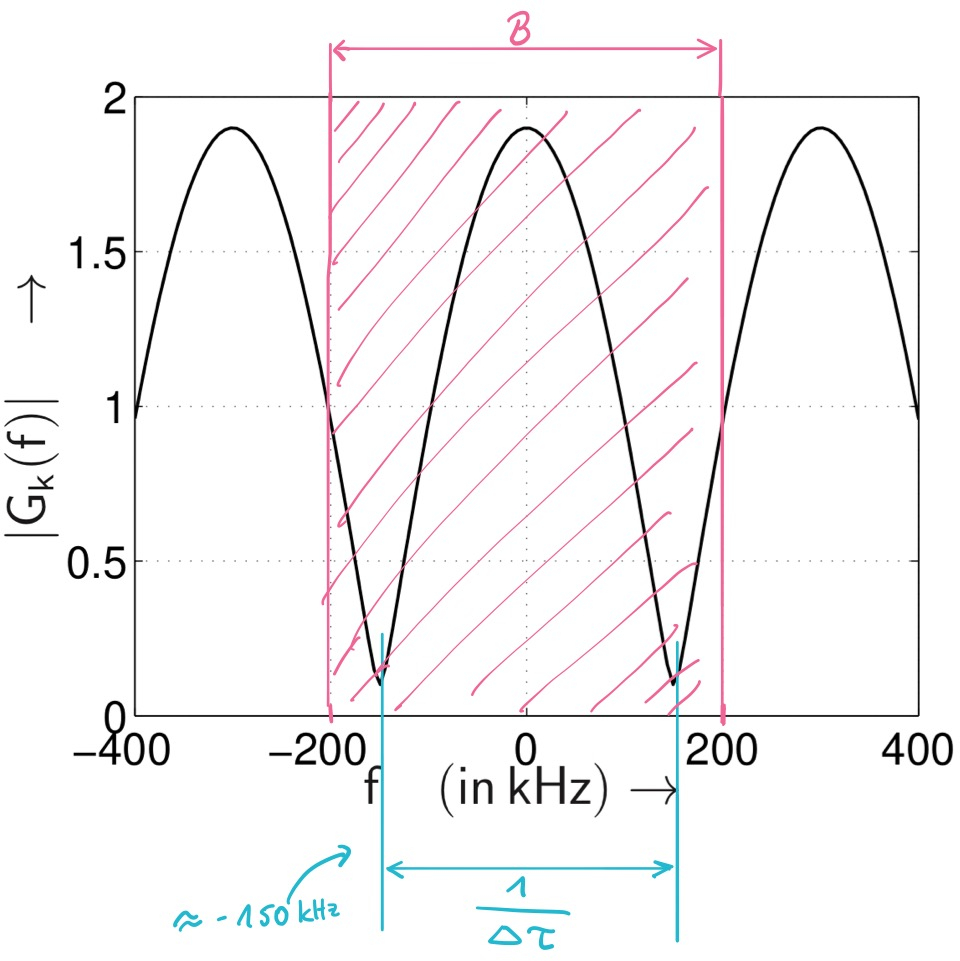
\includegraphics[width=\textwidth]{screenshots/Aufgabe6/1}
  \end{center}

}{

  \begin{center}
    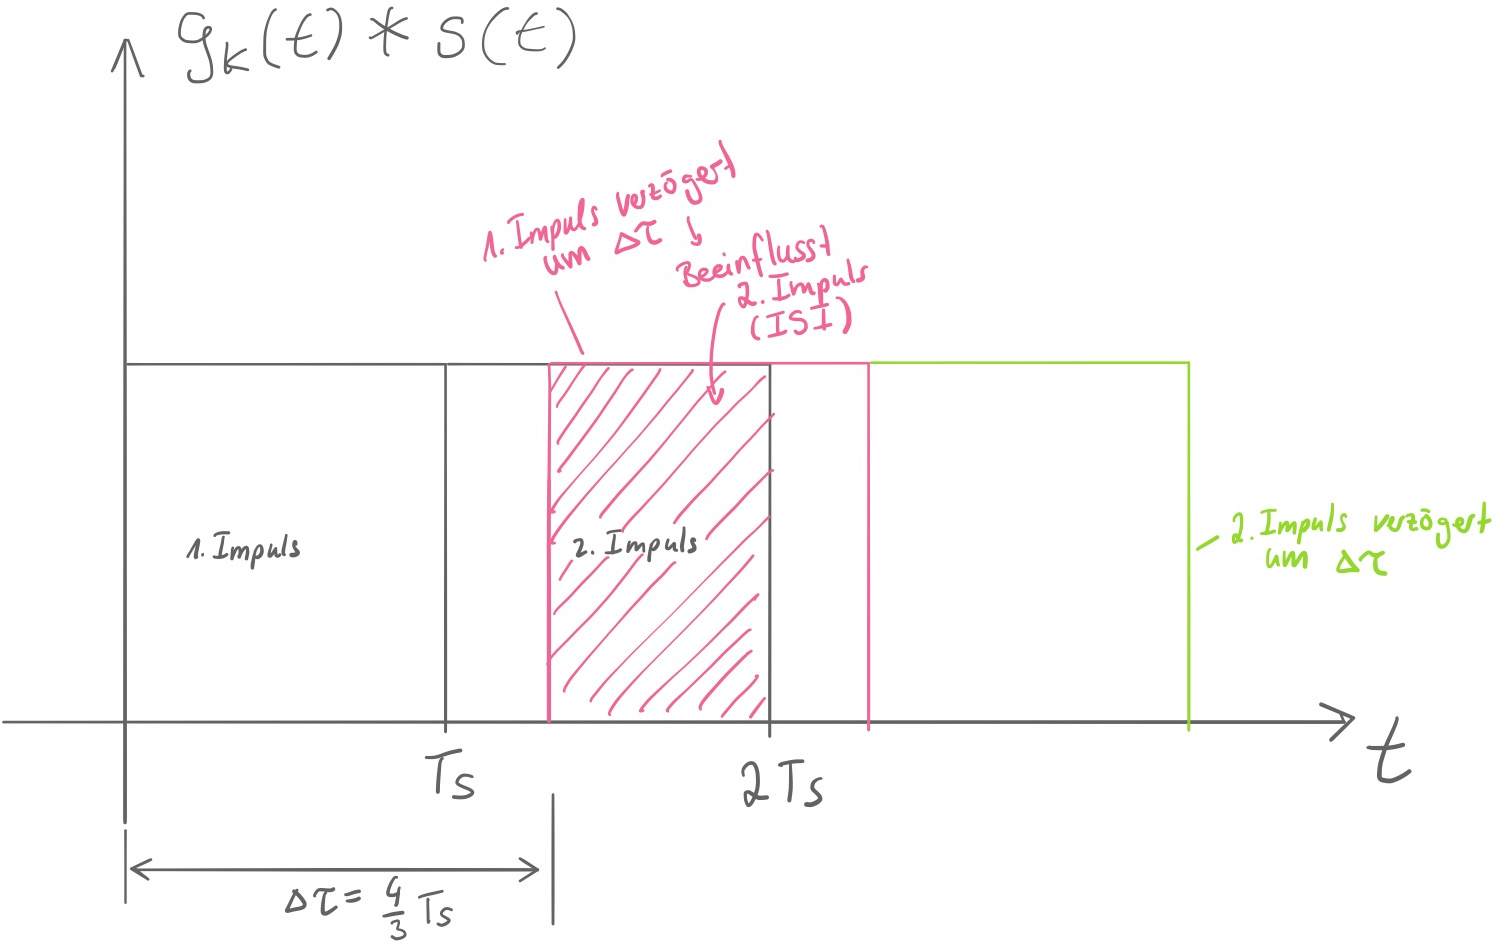
\includegraphics[width=\textwidth]{screenshots/Aufgabe6/2}
  \end{center}

  
}{0.5\textwidth}

\end{frame}

  \section{Aufgabe 6}
  \input{slides/Aufgabe6}

  \section{Aufgabe 7}
  \begin{frame}{Aufgabe 7}
  \begin{center}
  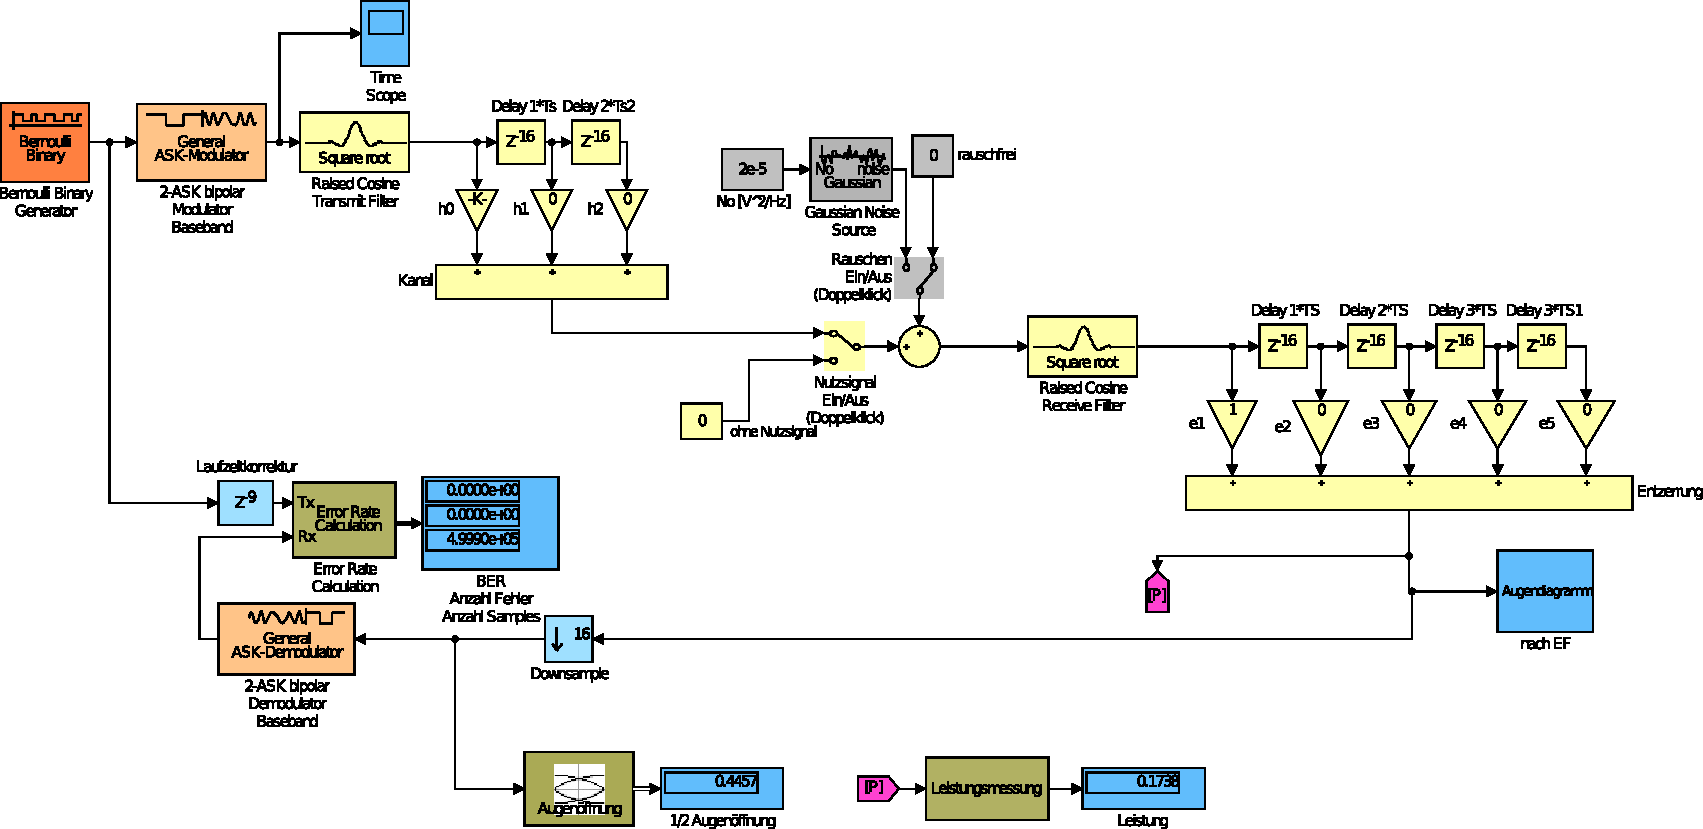
\includegraphics[width=\textwidth]{screenshots/Aufgabe7/modell}
  \end{center}
\end{frame}

\begin{frame}{Aufgabe 7}
  \[g_\mathrm{k}(t) = \frac{1}{\sqrt{5}} \cdot \delta(t)\]
\begin{table}[]
\begin{tabular}{
>{\columncolor{gray0}}l ll}
Kenngröße                          & \cellcolor{gray0}AWGN-Wert & \cellcolor{gray0}A7-Wert \\ \hline
$U_\mathrm{A}$                     & $0.9965 \, \si{\volt}$            & $0.4457 \, \si{\volt}$          \\
$U_\mathrm{R}^2$                   & $0.1 \, \si{\volt}^2$             & $0.1047 \, \si{\volt}^2$        \\
$\rho$                             & $9.93$                            & $1.897$                         \\
$\mathrm{BER}, \mathrm{berechnet}$ & $8.1303 \cdot 10^{-4}$            & $8.42 \cdot 10^{-2}$            \\
$\mathrm{BER}, \mathrm{gemessen}$  & $8.6315 \cdot 10^{-4}$            & $8.024 \cdot 10^{-2}$          
\end{tabular}
\end{table}
\end{frame}

  \section{Aufgabe 8}
  \begin{frame}{Aufgabe 8}
\begin{table}[]
\begin{tabular}{
>{\columncolor{gray0}}l ll}
Kenngröße                          & \cellcolor{gray0}Wert ohne Entzerrer    & \cellcolor{gray0}Wert mit Entzerrer       \\ \hline
$U_\mathrm{A}$                     & $0.4442 \, \si{\volt}$                         & \cellcolor{orange2}$0.9581 \, \si{\volt}$   \\
$U_\mathrm{R}^2$                   & $0.09136 \, \si{\volt}^2$                      & \cellcolor{orange2}$0.1452 \, \si{\volt}^2$ \\
$\rho$                             & $2.1597$                                       & $6.3220$                                         \\
$\mathrm{BER}, \mathrm{berechnet}$ & \cellcolor{red2}$7.08 \cdot 10^{-2}$   & $6.0 \cdot 10^{-3}$                              \\
$\mathrm{BER}, \mathrm{gemessen}$  & \cellcolor{red2}$3.9887 \cdot 10^{-2}$ & $7.3382 \cdot 10^{-3}$                          
\end{tabular}
\end{table}
\end{frame}

\begin{frame}{Aufgabe 8: Nyquistvektor}

  Veränderung  der Position der 1 im Nyquistvektor
  \smallgrskip

  Qualitätskriterium:
  \to Summe der quadratischen Abweichungen der Faltung {\color{cyan5}{$h(k) * f(k)$}} zu dem Nyquistvektor {\color{cyan5}{$z(k)$}}

  \smallgrskip
  \[ \sum(h(k) * f(k) - z(k) ) ^2 \rightarrow min\]

\end{frame}

\begin{frame}{Aufgabe 8: Augendiagramme}

  \twocolumns{
  \begin{center}
  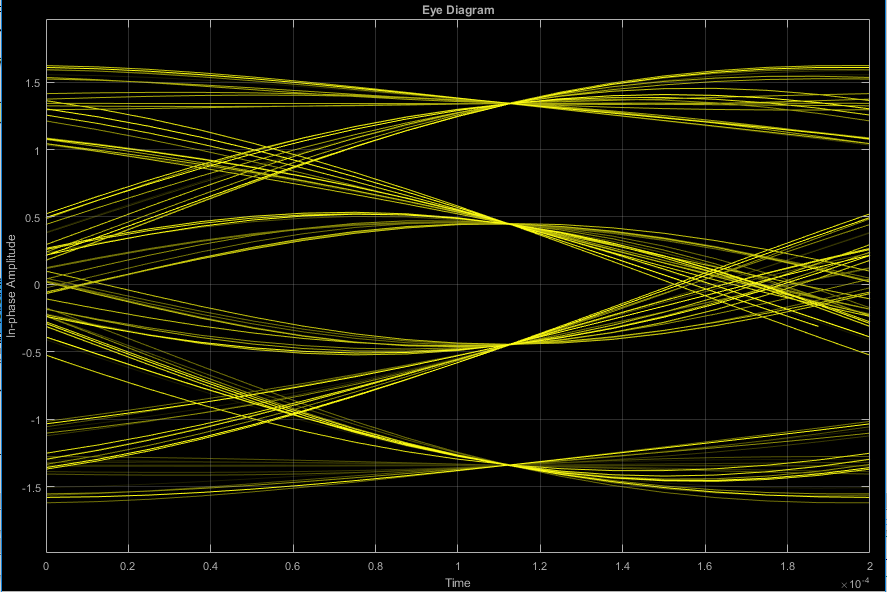
\includegraphics[width=\textwidth]{screenshots/Aufgabe8/Auge_ohne_entzerrer}
  \end{center}
} {
  \begin{center}
  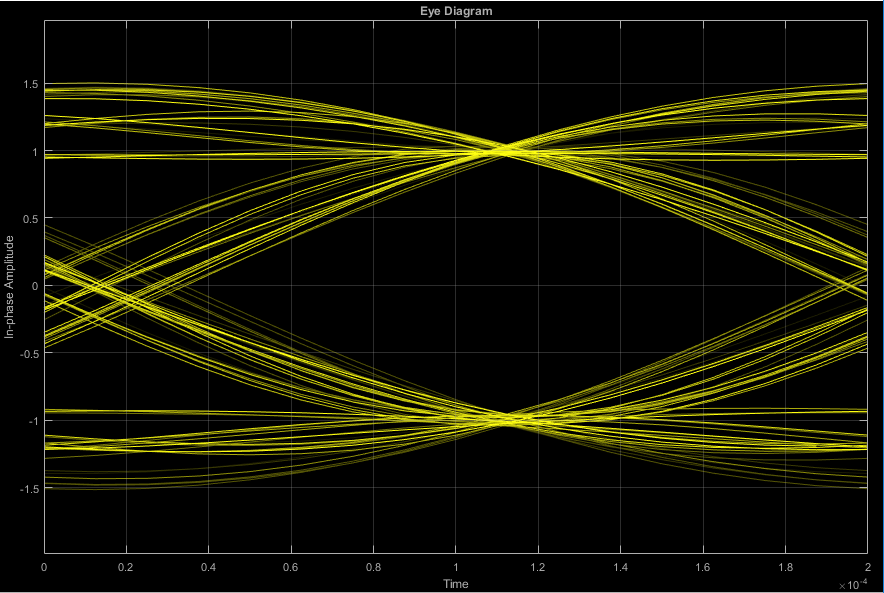
\includegraphics[width=\textwidth]{screenshots/Aufgabe8/Auge_mit_entzerrer}
  \end{center}
  
}{0.5\textwidth}
\end{frame}

\begin{frame}{Aufgabe 8: Rauschleistungsanhebung}
  \[\sum{f_i^2} = 1.654\]
\end{frame}

\begin{frame}{Aufgabe 8: BER-Vergleich}

  \twocolumns{
 Einstellung
    von $N_0$ im \textsc{SIMULINK}-Modell 
    \smallgrskip

    \[ \mathrm{SNR}_\mathrm{dB} = 10 \cdot \log_{10}{\frac{E_\mathrm{s}}{N_0}}\]

    \[N_0 = \frac{E_\mathrm{s}}{10^{\frac{\mathrm{SNR}}{10}}}\]

  }{

  \begin{center}
  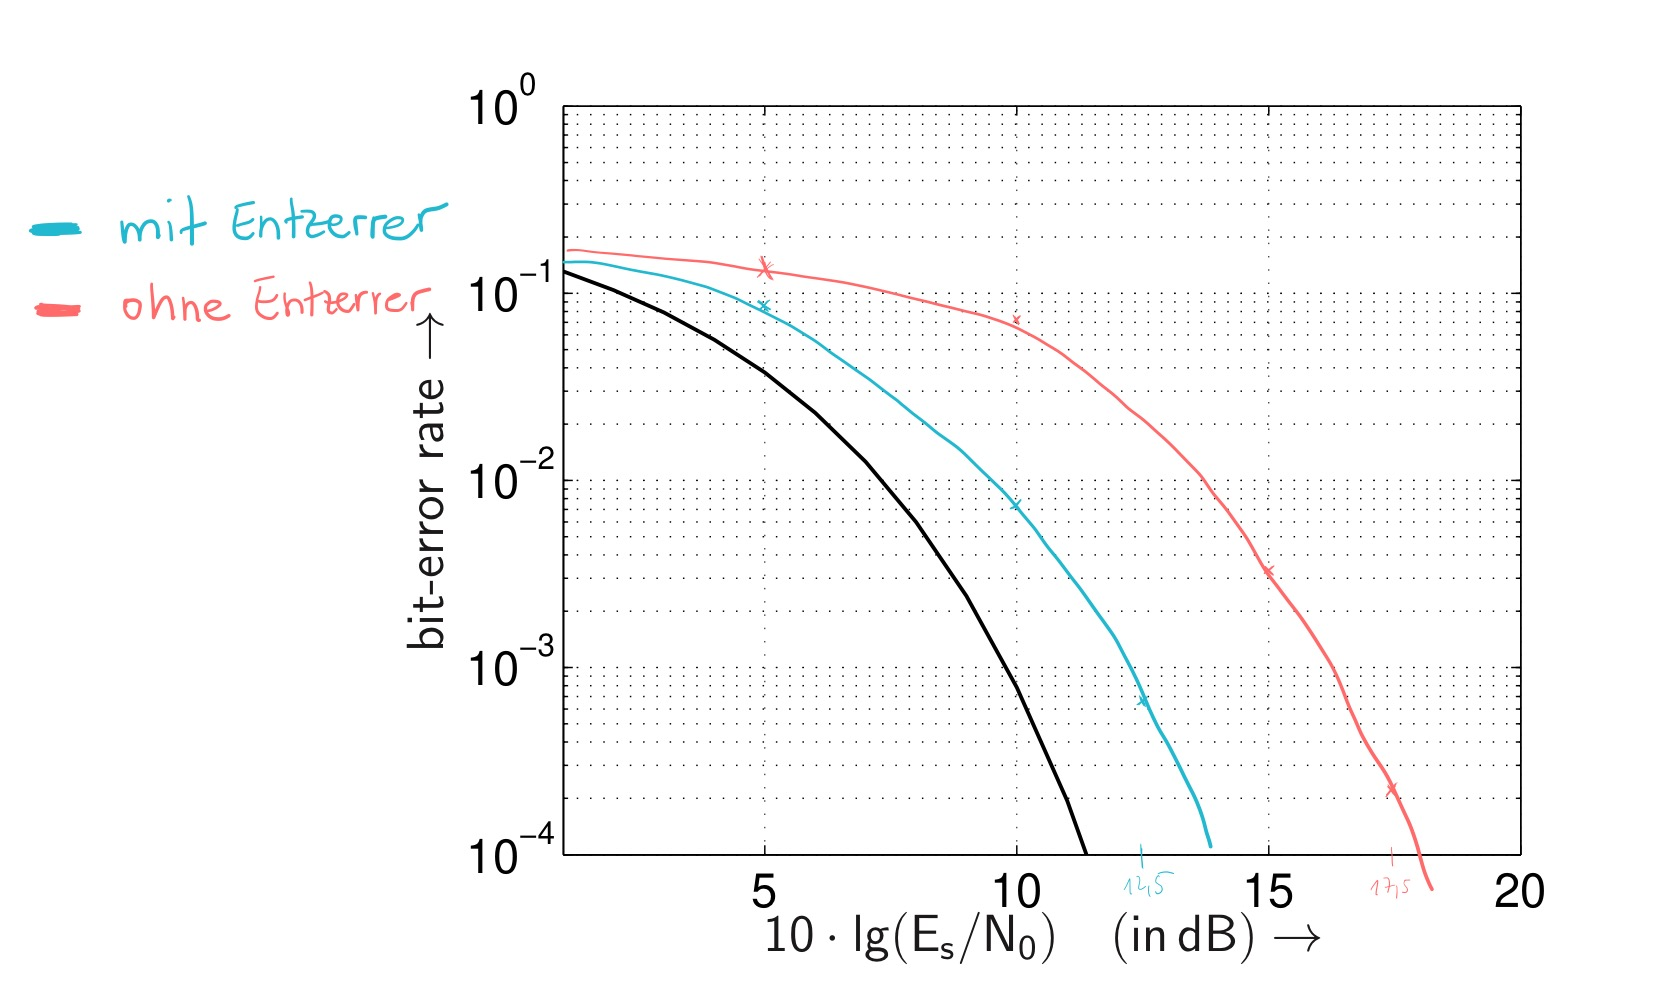
\includegraphics[width=\textwidth]{screenshots/Aufgabe8/BER}
  \end{center}

  }{0.382\textwidth}
  
\end{frame}



  \section{Aufgabe 9}
  \begin{frame}{Aufgabe 9}

  \twocolumns{

    \begin{center}
      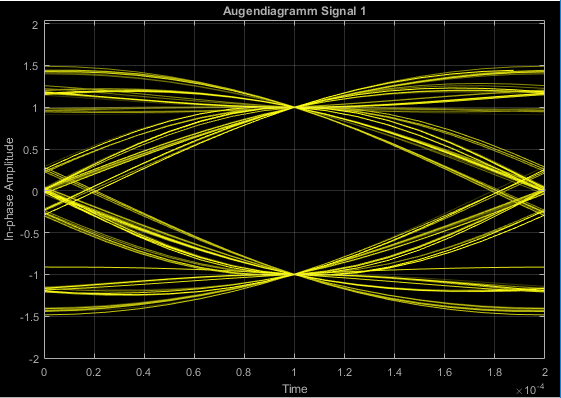
\includegraphics[width=\textwidth]{screenshots/Aufgabe9/Augendiagramm1}
    \end{center}

  }{
    \begin{center}
      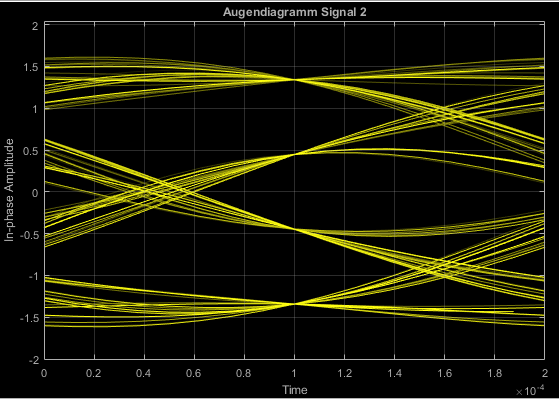
\includegraphics[width=\textwidth]{screenshots/Aufgabe9/Augendiagramm2}
    \end{center}

  }{0.5\textwidth}

\end{frame}
  
\end{document}